\documentclass[conference]{IEEEtran}
\usepackage{graphicx}
\usepackage{amsmath}
\usepackage{cite}
\usepackage{url}
\usepackage{booktabs}
\usepackage{float}

\title{Exploring Economic Data and Its Impact on Unemployment Rates}

\author{
    \IEEEauthorblockN{Ali Mansouri\IEEEauthorrefmark{1}, Malhar Jojare\IEEEauthorrefmark{2}}
    \IEEEauthorblockA{
        \IEEEauthorrefmark{1}Civil, Environmental, and Geospatial Engineering Department, Michigan Technological University, Houghton, USA \\
        Email: alimanso@mtu.edu
    }
    \IEEEauthorblockA{
        \IEEEauthorrefmark{2}College of Computing, Michigan Technological University, Houghton, USA \\
        Email: msjojare@mtu.edu
    }
}

\begin{document}
\maketitle

\begin{abstract}
This study investigates the relationship between key macroeconomic indicators and the unemployment rate in the United States over the period 1974 to 2023. Using historical data from the World Bank, the analysis focuses on five economic variables: GDP (current US\$), GDP growth, real interest rate, inflation, and unemployment. The dataset was preprocessed and analyzed using both statistical and machine learning techniques, including correlation analysis, time-series smoothing, and regression modeling. Among the predictive models tested, the Random Forest Regressor demonstrated the highest accuracy, explaining approximately 31\% of the variance in unemployment. Feature importance analysis revealed that GDP and GDP growth were the strongest predictors. The findings support the presence of long-term economic patterns influencing unemployment and highlight the utility of combining data-driven approaches with economic theory for policy insights and future forecasting.
\end{abstract}

\begin{IEEEkeywords}
Unemployment, Economic Indicators, GDP Growth, Inflation, Labor Market, Data Science, Time-Series Analysis, Machine Learning
\end{IEEEkeywords}

\section{Introduction}
Unemployment rates serve as a crucial measure of economic well-being, impacting individuals, businesses, and governments alike. Understanding the underlying factors driving unemployment is essential for policy formulation, economic planning, and crisis management. This study investigates how macroeconomic indicators—including GDP, interest rates, inflation, and GDP growth—have influenced the U.S. unemployment rate from 1974 to 2023. By analyzing historical economic data and applying predictive modeling techniques, the research aims to identify long-term trends and key predictors that can inform efforts to mitigate unemployment risks and promote economic stability.

\section{Literature Review}
Several studies have examined the relationship between macroeconomic indicators and unemployment. Smith et al.~\cite{smith2021economic} found an inverse correlation between GDP growth and unemployment (Okun’s Law) but did not account for structural unemployment factors. Jones and Lee~\cite{jones2019predicting} employed machine learning models using inflation, interest rates, and consumer confidence indices to predict unemployment trends with high accuracy, though at the expense of interpretability. Brown et al.~\cite{brown2022unemployment} analyzed unemployment trends during economic crises, showing that specific demographic groups faced disproportionate impacts. However, their study focused on short-term effects rather than long-term macroeconomic trends. Our study builds on these findings by combining statistical analysis and data science techniques to uncover long-term economic drivers of unemployment.

\section{Methodology and Results}
\subsection{Data Collection and Preprocessing}

For this project, we collected macroeconomic data from the World Bank, spanning from 1974 to 2023, and selected five key economic indicators relevant to analyzing unemployment trends:
\begin{itemize}
    \item GDP (current US\$)
    \item GDP growth (annual \%)
    \item Unemployment, total (\% of total labor force)
    \item Real interest rate (\%)
    \item Inflation, consumer prices (annual \%)
\end{itemize}

The original dataset covered 266 countries, with 1,332 rows and 54 columns. The first four columns contained metadata (series and country information), while the remaining 50 columns represented annual values.

To narrow our focus, we filtered the dataset to include only data for the United States. This decision was based on the goal of analyzing the dynamic relationship between economic performance and unemployment within a single, stable economic context.

To prepare the dataset for analysis, we followed a series of preprocessing steps designed to clean, restructure, and format the data for time-series modeling.

\subsubsection{Preprocessing Steps}

\begin{itemize}
    \item \textbf{Missing Data Identification and Handling:} Replaced placeholder missing values (‘..’) with \texttt{NaN} to standardize handling. Since only two rows had missing data, they were dropped to maintain data integrity without losing significant information.

    \item \textbf{Data Restructuring:} Removed metadata columns and transposed the dataset. This conversion turned economic indicators into columns and years into rows, enabling intuitive time-series analysis.

    \item \textbf{Year Formatting:} Used regular expressions to extract four-digit years from labels such as \texttt{1974 [YR1974]} and converted them to integers. This facilitated sorting and visualizations across time.
\end{itemize}
\begin{table}[ht]
\caption{Descriptive Statistics of Dataset (1974–2023)}
\label{tab:stats}
\centering
\begin{tabular}{@{}lccccc@{}}
\toprule
Indicator & Mean & Std & Min & 25\% & Max \\
\midrule
GDP (\$) & 1.00E+13 & 6.36E+12 & 1.55E+12 & 4.52E+12 & 2.37E+13 \\
Unemp. (\%) & 6.30 & 1.61 & 3.67 & 5.23 & 9.70 \\
Int. Rate (\%) & 3.98 & 2.46 & -1.28 & 2.08 & 8.59 \\
GDP Growth (\%) & 2.68 & 2.07 & -2.58 & 1.87 & 7.24 \\
Inflation (\%) & 3.88 & 2.95 & -0.36 & 2.11 & 13.55 \\
\bottomrule
\end{tabular}
\end{table}

Table~\ref{tab:stats} provides a summary of the dataset after pre-processing, highlighting key statistics such as mean, standard deviation, and quartiles for each economic indicator. A few noteworthy insights include:
\begin{itemize}
    \item GDP has grown significantly, from a minimum of \$1.55 trillion to a maximum of \$23.7 trillion, reflecting long-term economic expansion.
    \item Unemployment fluctuated between 3.67\% and 9.7\%, with a mean of 6.3\%, giving context for recession and recovery periods.
    \item Inflation and interest rates show considerable variability (with inflation peaking at 13.55\%), often correlating with macroeconomic instability and policy changes.
    \item GDP growth ranges from strong contractions (-2.58\%) to expansions (7.24\%), emphasizing the cyclical nature of economic performance.
\end{itemize}

These statistics provide foundational context for visualizations and machine learning models in the following sections of the report, helping interpret how each economic factor influences unemployment trends.

\subsection{Exploratory Data Analysis (EDA)}

To better understand the behavior of each economic indicator and uncover potential patterns influencing unemployment, we performed both visual and statistical exploratory analysis.

\subsubsection*{Kernel Density Estimation (KDE) \textendash{} Distribution Analysis}
We applied Kernel Density Estimation (KDE) to generate smooth probability distributions for all five economic indicators. This approach helps visualize how each variable is distributed across the dataset, especially after scaling the values to a uniform range for comparison. Figure~\ref{fig:kde} illustrates the KDE plots for economic indicators.

From the KDE plots in Figure~\ref{fig:kde}, we observe that:
Unemployment rate has a sharp and concentrated peak compared to other variables, suggesting less variability over time.
Inflation also exhibits sharply peaked and a slightly skewed distribution, indicating occasional extreme values (e.g., during economic crises).
GDP growth and real interest rates have wider distributions, highlighting their fluctuating nature across the decades.
GDP follows a more moderately dispersed pattern, reflecting steady but exponential economic growth over time.
These distribution patterns are critical in identifying data spread, and skewness, and they provide early hints about potential correlations (e.g., whether higher inflation corresponds with unemployment spikes). This analysis lays the groundwork for further correlation studies.

\begin{figure}[H]
    \centering
    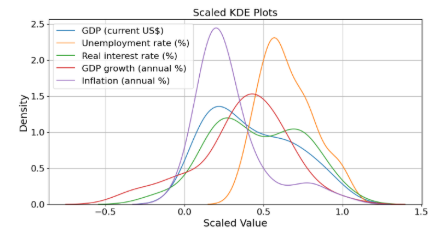
\includegraphics[width=0.9\linewidth]{kde_plot.png}
    \caption{Scaled KDE Plots of parameters}
    \label{fig:kde}
\end{figure}
\vspace*{-1.3em}

\subsubsection*{Correlation Analysis}
To explore how economic indicators relate to one another\textemdash especially in terms of their influence on unemployment\textemdash we computed the Pearson correlation matrix. This method quantifies the linear relationship between each pair of variables, with values ranging from -1 (perfect inverse correlation) to +1 (perfect direct correlation). Fig.~\ref{fig:correlation} presents a heatmap revealing key correlations.

Key findings from the correlation matrix include:
Inflation and GDP exhibit a strong negative correlation (-0.63), indicating that periods of higher inflation often correspond with slower economic growth or declining output. This may reflect stagflation or contractionary monetary responses.
GDP growth and unemployment maintain a moderate negative correlation (-0.30), reinforcing the idea that stronger economic performance tends to reduce joblessness.
GDP and unemployment also show an inverse correlation (-0.29), supporting the general macroeconomic trend that higher national income levels are associated with lower unemployment.
Real interest rates have a mild negative correlation with GDP (-0.43) and weak associations with other indicators, implying indirect or lagged effects on economic performance.
Inflation and unemployment display a weak positive correlation (0.14)\textemdash suggesting that inflationary periods may slightly increase unemployment, although the relationship is not strongly linear in this dataset.

\begin{figure}[H]
    \centering
    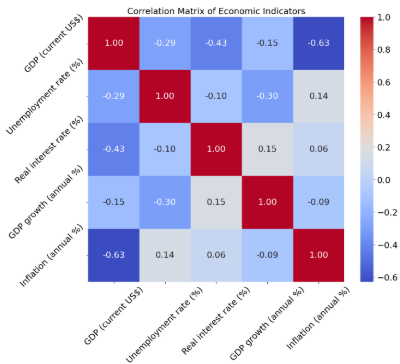
\includegraphics[width=0.9\linewidth]{correlation_matrix.png}
    \caption{Correlation Matrix of Economic Indicators}
    \label{fig:correlation}
\end{figure}
\vspace{-10pt}


\subsubsection*{Time-Series Analysis}
To better capture long-term economic trends and reduce short-term fluctuations, we applied 5-year moving averages (MA) to each indicator. This smoothing technique helps reveal persistent patterns and relationships that may influence unemployment over time. Figures~\ref{fig:gdp_growth_ma}--\ref{fig:all_indicators} show the original and smoothed trends of key economic variables from 1974 to 2021. These visualizations highlight trends such as the economic downturn during the 2008 crisis, inflationary periods, and the impact of interest rate fluctuations.

Fig.~\ref{fig:gdp_growth_ma} exhibits high short-term variability of GDP growth. The smoothed line captures growth cycles, with notable dips during recessions (e.g., early 80s, 2008, and 2020), and moderate growth during recoveries.

\begin{figure}[H]
    \centering
    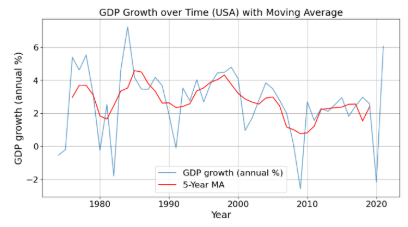
\includegraphics[width=0.9\linewidth]{gdp_growth_ma.png}
    \caption{GDP Growth over Time (USA) with Moving Average}
    \label{fig:gdp_growth_ma}
\end{figure}

Fig.~\ref{fig:interest_rate} shows that real interest rate rose sharply in the late 1970s and early 1980s, coinciding with efforts to combat high inflation. The downward trend since the 1990s reflects more accommodative monetary policies.

\begin{figure}[H]
    \centering
    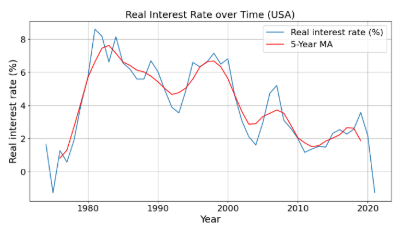
\includegraphics[width=0.9\linewidth]{interest_rate.png}
    \caption{Real Interest Rate over Time (USA)}
    \label{fig:interest_rate}
\end{figure}

Fig.~\ref{fig:unemployment} reflects cyclical spikes of unemployment rate corresponding to recessions (early 1980s, 2008, and 2020). The MA smooths these spikes, indicating long-term unemployment hovered around 5--6\%, with notable declines in the mid-1990s and late 2010s.

\begin{figure}[H]
    \centering
    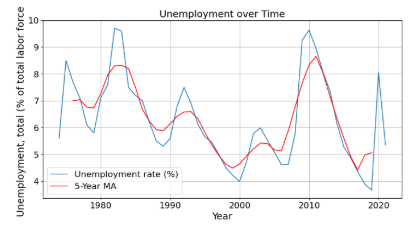
\includegraphics[width=0.9\linewidth]{unemployment.png}
    \caption{Unemployment over Time}
    \label{fig:unemployment}
\end{figure}

Fig.~\ref{fig:inflation} shows high volatility of inflation in the 1970s and early 1980s, with peaking near 13\%, then tapering to more stable rates from the 1990s onward. The moving average line highlights long-term disinflation trends.

\begin{figure}[htbp]
    \centering
    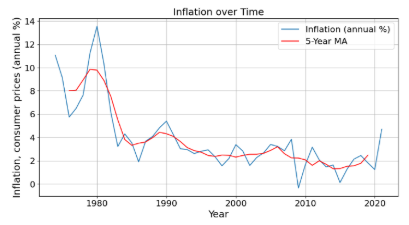
\includegraphics[width=0.9\linewidth]{inflation.png}
    \caption{Inflation over Time}
    \label{fig:inflation}
\end{figure}

Fig.~\ref{fig:gdp_total} demonstrates a strong and steady increase of GDP in the U.S. economy's output, especially post-1990, with brief flattening around the 2008 financial crisis and COVID-19 pandemic.

\begin{figure}[htbp]
    \centering
    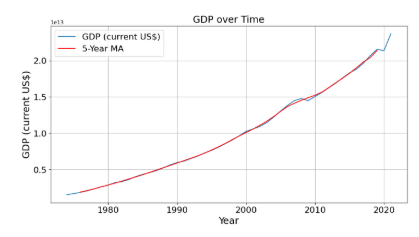
\includegraphics[width=0.9\linewidth]{gdp_total.png}
    \caption{GDP over Time}
    \label{fig:gdp_total}
\end{figure}

Fig.~\ref{fig:all_indicators} displays a comprehensive view of all indicators over time. While GDP shows a steady upward trajectory, unemployment, inflation, and interest rates clearly exhibit cyclical behaviours. This plot offers an integrated look at how economic health and volatility have evolved together.

\begin{figure}[htbp]
    \centering
    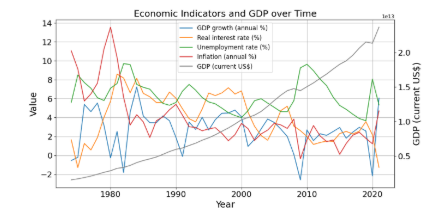
\includegraphics[width=0.9\linewidth]{all_indicators.png}
    \caption{Economic Indicators and GDP over Time}
    \label{fig:all_indicators}
\end{figure}

\subsection{Predictive Modeling}

To quantify how macroeconomic indicators influence the U.S. unemployment rate, we built and evaluated several regression models. Our goal was to predict unemployment using the following predictors:
\begin{itemize}
    \item GDP (current US\$)
    \item GDP growth (annual \%)
    \item Real interest rate (\%)
    \item Inflation (annual \%)
\end{itemize}

The dataset was split into 80\% training and 20\% testing subsets to validate performance.

\subsubsection*{Regression Results}
We evaluated models using standard metrics: Mean Squared Error (MSE), Root Mean Squared Error (RMSE), Mean Absolute Error (MAE), Mean Absolute Percentage Error (MAPE), and R-squared (R\textsuperscript{2}). Table~\ref{tab:regression} summarizes the performance of each regression model across key evaluation metrics.

\begin{table}[htbp]
    \centering
    \caption{Model Performance Comparison}
    \label{tab:regression}
    \resizebox{\linewidth}{!}{%
    \begin{tabular}{lccccc}
        \toprule
        Model & MSE & RMSE & MAE & MAPE (\%) & R\textsuperscript{2} \\
        \midrule
        Linear Regression & 2.189 & 1.48 & 1.21 & 23.8 & 0.062 \\
        Decision Tree Regressor & 2.691 & 1.64 & 1.318 & 22.06 & -0.153 \\
        Random Forest Regressor & 1.615 & 1.271 & 1.168 & 22.74 & 0.308 \\
        Random Forest (GridSearchCV) & 1.621 & 1.273 & 1.147 & 22.4 & 0.306 \\
        \bottomrule
    \end{tabular}
    }
\end{table}
\textbf{Linear Regression:} The baseline linear model revealed limited predictive strength, R\textsuperscript{2} = 0.06, indicating that only 6\% of unemployment variation is explained by the model. While the MAPE (\textasciitilde23.8\%) is within a tolerable range, the model underperforms in capturing complex, nonlinear interactions among variables.

\textbf{Decision Tree Regressor:} Despite its ability to capture non-linearities, the model yielded R\textsuperscript{2} = -0.15, suggesting worse performance than simply using the mean. Both MSE and RMSE increased, with a slight improvement in MAPE (\textasciitilde22.1\%).

\textbf{Random Forest Regressor:} This ensemble model significantly improved performance, R\textsuperscript{2} = 0.31, explaining approximately 31\% of the variance. RMSE = 1.27 and MAPE = 22.7\% were notably better than previous models.

\textbf{Random Forest with GridSearchCV (Tuned Model):} After hyperparameter tuning using GridSearchCV, the model achieved slightly better generalization, R\textsuperscript{2} = 0.31, MAPE = 22.4\%. This version confirmed Random Forest as the most effective model for our data.

\subsubsection*{Feature Importance}
As shown in Figure~\ref{fig:feature_importance}, the Random Forest model revealed that:
\begin{itemize}
    \item GDP (current US\$) is the most influential variable
    \item Followed by GDP growth and real interest rate
    \item Inflation, while still relevant, contributed the least predictive power
\end{itemize}
This ranking aligns with economic theory: stronger output and growth often correlate with better labor market conditions, while inflation may affect unemployment more indirectly or cyclically.

\subsubsection*{Classification Results}
To provide a categorical indication of the degree of unemployment, classification models were developed. The output classes were \textbf{Low}, \textbf{Moderate}, and \textbf{High} unemployment. Precision, recall, F1-score, and accuracy were utilized to evaluate performance. The confusion matrix (Figure~\ref{fig:confusion_matrix}) and metrics are as follows.

\begin{figure}[htbp]
    \centering
    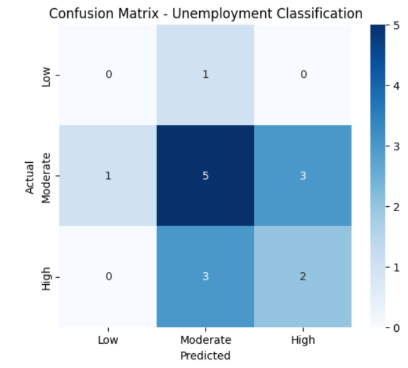
\includegraphics[width=0.85\linewidth]{confusion_matrix.png}
    \caption{Confusion Matrix Unemployment Classification}
    \label{fig:confusion_matrix}
\end{figure}

\textbf{Classification Performance -- Random Forest Classifier}
\begin{table}[htbp]
    \centering
    \begin{tabular}{lcccc}
        \toprule
        Class & Precision & Recall & F1-Score & Support \\
        \midrule
        High & 0.4 & 0.4 & 0.4 & 5 \\
        Low & 0 & 0 & 0 & 1 \\
        Moderate & 0.6 & 0.667 & 0.632 & 9 \\
        \midrule
        Accuracy & \multicolumn{4}{c}{0.533 (15 instances)} \\
        Macro avg & 0.333 & 0.356 & 0.344 & \\
        Weighted avg & 0.493 & 0.533 & 0.512 & \\
        \bottomrule
    \end{tabular}
\end{table}

The Random Forest classifier yielded the best accuracy (53.3\%) and outperformed the baseline model (46.7\%). The Moderate class was the most reliably predicted, whereas performance for the Low class was notably poor due to class imbalance (only one instance in the test set).
\subsubsection*{Confusion Matrix Analysis}
As illustrated in Fig.~\ref{fig:confusion_matrix}, the confusion matrix revealed that:
\begin{itemize}
    \item 5 out of 9 Moderate unemployment instances were correctly classified.
    \item Misclassifications were most frequent between Moderate and High categories.
    \item The model failed to identify the Low class, reinforcing the need for rebalancing techniques such as oversampling or synthetic data generation in future work.
\end{itemize}

While the models do not fully explain unemployment variation\textemdash likely due to unobserved external shocks, policy shifts, or lag effects\textemdash the Random Forest Regressor offered the best predictive performance. The results reinforce the importance of GDP-related metrics in forecasting employment trends and highlight opportunities to enhance accuracy by incorporating lag variables or broader socio-economic factors in future work.


\section{Conclusion}

This project explored the relationship between macroeconomic indicators and the U.S. unemployment rate over the period from 1974 to 2023 using data from the World Bank. Through a combination of exploratory data analysis, correlation studies, and predictive modeling, we gained valuable insights into how economic trends align with changes in employment.

Key takeaways include:
\begin{itemize}
    \item GDP and GDP growth are consistently the strongest indicators influencing unemployment, both statistically and in predictive models.
    \item Unemployment exhibits a cyclical pattern that corresponds with economic downturns, such as the early 1980s, the 2008 financial crisis, and the 2020 pandemic.
    \item Inflation and interest rates, while important in macroeconomic contexts, showed weaker direct predictive power for unemployment in this dataset.
    \item The Random Forest Regressor, especially after hyperparameter tuning, provided the best modeling results, explaining approximately 31\% of the variance in unemployment rates.
\end{itemize}

While the results are meaningful, the models could benefit from the inclusion of additional predictors (e.g., labor market participation, government spending) and lag features that account for delayed effects of economic policy. Future work could also explore deep learning or time-series-specific approaches (e.g., ARIMA, LSTM) for more robust forecasting.

\section*{Acknowledgment}
We thank Michigan Technological University for providing access to necessary resources and datasets.

\bibliographystyle{IEEEtran}
\bibliography{refs}
\section*{Self-Declaration of Contributions}

\textbf{Ali Mansouri (alimanso@mtu.edu)}\\
I was responsible for collecting and preprocessing the macroeconomic dataset from the World Bank. I also conducted exploratory data analysis (EDA), including generating KDE plots, time-series smoothing, and correlation matrices. Additionally, I contributed to writing the introduction and data analysis sections of the report.

\vspace{1em}

\textbf{Malhar Jojare (msjojare@mtu.edu)}\\
I developed and evaluated the regression and classification models, including hyperparameter tuning with GridSearchCV. I performed the feature importance analysis and created the visualizations for model evaluation. I also contributed to writing the predictive modeling and conclusion sections of the report.

\end{document}
